\documentclass[10pt,a4paper,onecolumn]{article}
% \usepackage[utf8]{inputenc}
\usepackage{marginnote}
\usepackage{graphicx}
\usepackage{xcolor}
\usepackage{authblk,etoolbox}
\usepackage{titlesec}
\usepackage{calc}
\usepackage{hyperref}
\hypersetup{breaklinks=true,
            bookmarks=true,
            pdfauthor=
{
      Erwan Le Masson,
      Frédéric Alexandre,
  },
            pdftitle=
{
[Re] How Attention Can Create Synaptic Tags for the Learning of Working
Memories in Sequential Tasks
},
            colorlinks=true,
            citecolor=blue,
            urlcolor=blue,
            linkcolor=blue,
            pdfborder={0 0 0}}
\urlstyle{same}
\usepackage{tcolorbox}
\usepackage{ragged2e}
\usepackage{fontspec}
\usepackage{fontawesome}
\usepackage{caption}
\usepackage{listings}
\lstnewenvironment{code}{\lstset{language=Haskell,basicstyle=\small\ttfamily}}{}



%\usepackage{fancyvrb}
%\VerbatimFootnotes
%\usepackage{graphicx}
%\usepackage{mdframed}
%\newmdenv[backgroundcolor=lightgray]{Shaded}


\usepackage{longtable,booktabs}

\usepackage[
  backend=biber,
%  style=alphabetic,
%  citestyle=numeric
]{biblatex}
\bibliography{Le_Masson-Alexandre-2016.bib}



% --- Macros ------------------------------------------------------------------
\renewcommand*{\bibfont}{\small \sffamily}

\definecolor{red}{HTML}{CF232B}
\newcommand{\ReScience}{Re{\bfseries \textcolor{red}{Science}}}

\newtcolorbox{rebox}
   {colback=blue!5!white, colframe=blue!40!white,
     boxrule=0.5pt, arc=2pt, fonttitle=\sffamily\scshape\bfseries,
     left=6pt, right=20pt, top=6pt, bottom=6pt}

\newtcolorbox{repobox}
   {colback=red, colframe=red!75!black,
     boxrule=0.5pt, arc=2pt, left=6pt, right=6pt, top=3pt, bottom=3pt}

% fix for pandoc 1.14     
\newcommand{\tightlist}{%
  \setlength{\itemsep}{1pt}\setlength{\parskip}{0pt}\setlength{\parsep}{0pt}}

% --- Style -------------------------------------------------------------------
\renewcommand*{\bibfont}{\small \sffamily}
\renewcommand{\captionfont}{\small\sffamily}
\renewcommand{\captionlabelfont}{\bfseries}

\makeatletter
\renewcommand\@biblabel[1]{{\bf #1.}}
\makeatother

% --- Page layout -------------------------------------------------------------
\usepackage[top=3.5cm, bottom=3cm, right=1.5cm, left=1.5cm,
            headheight=2.2cm, reversemp, includemp, marginparwidth=4.5cm]{geometry}

% --- Section/SubSection/SubSubSection ----------------------------------------
\titleformat{\section}
  {\normalfont\sffamily\Large\bfseries}
  {}{0pt}{}
\titleformat{\subsection}
  {\normalfont\sffamily\large\bfseries}
  {}{0pt}{}
\titleformat{\subsubsection}
  {\normalfont\sffamily\bfseries}
  {}{0pt}{}
\titleformat*{\paragraph}
  {\sffamily\normalsize}


% --- Header / Footer ---------------------------------------------------------
\usepackage{fancyhdr}
\pagestyle{fancy}
%\renewcommand{\headrulewidth}{0.50pt}
\renewcommand{\headrulewidth}{0pt}
\fancyhead[L]{\hspace{-1cm}\includegraphics[width=4.0cm]{rescience-logo.pdf}}
\fancyhead[C]{}
\fancyhead[R]{} 
\renewcommand{\footrulewidth}{0.25pt}

\fancyfoot[L]{\hypersetup{urlcolor=red}
              \sffamily \ReScience~$\vert$
              \href{http://rescience.github.io}{rescience.github.io}
              \hypersetup{urlcolor=blue}}
\fancyfoot[C]{\sffamily \thepage}
\fancyfoot[R]{\sffamily Dec 2016 $\vert$
                        Volume \textbf{2} $\vert$
                        Issue \textbf{1}}
\pagestyle{fancy}
\makeatletter
\let\ps@plain\ps@fancy
\fancyheadoffset[L]{4.5cm}
\fancyfootoffset[L]{4.5cm}

% --- Title / Authors ---------------------------------------------------------
% patch \maketitle so that it doesn't center
\patchcmd{\@maketitle}{center}{flushleft}{}{}
\patchcmd{\@maketitle}{center}{flushleft}{}{}
% patch \maketitle so that the font size for the title is normal
\patchcmd{\@maketitle}{\LARGE}{\LARGE\sffamily}{}{}
% patch the patch by authblk so that the author block is flush left
\def\maketitle{{%
  \renewenvironment{tabular}[2][]
    {\begin{flushleft}}
    {\end{flushleft}}
  \AB@maketitle}}
\makeatletter
\renewcommand\AB@affilsepx{ \protect\Affilfont}
%\renewcommand\AB@affilnote[1]{{\bfseries #1}\hspace{2pt}}
\renewcommand\AB@affilnote[1]{{\bfseries #1}\hspace{3pt}}
\makeatother
\renewcommand\Authfont{\sffamily\bfseries}
\renewcommand\Affilfont{\sffamily\small\mdseries}
\setlength{\affilsep}{1em}

\LetLtxMacro{\OldIncludegraphics}{\includegraphics}
\renewcommand{\includegraphics}[2][]{\OldIncludegraphics[width=12cm, #1]{#2}}


% --- Document ----------------------------------------------------------------
\title{[Re] How Attention Can Create Synaptic Tags for the Learning of Working
Memories in Sequential Tasks}

    \usepackage{authblk}
                        \author[1, 2, 3]{Erwan Le Masson}
                    \author[2, 1, 3]{Frédéric Alexandre}
                            \affil[1]{LaBRI, Université de Bordeaux, Bordeaux INP, CNRS, UMR 5800, Talence,
France}
                    \affil[2]{INRIA Bordeaux Sud-Ouest, 200 Avenue de la Vieille Tour, 33405 Talence,
France}
                    \affil[3]{IMN, Université de Bordeaux, CNRS, UMR 5293, Bordeaux, France}
            
\date{\vspace{-5mm}
      \sffamily \small \href{mailto:frederic.alexandre@inria.fr}{frederic.alexandre@inria.fr}}


\setlength\LTleft{0pt}
\setlength\LTright{0pt}


\begin{document}
\maketitle

\marginpar{
  %\hrule
  \sffamily\small
  %\vspace{2mm}
  {\bfseries Editor}\\
  Olivia Guest\\

  {\bfseries Reviewers}\\
        Julien Vitay\\
        Etienne Roesch\\
  
  {\bfseries Received}  Aug, 9, 2016\\
  {\bfseries Accepted}  Dec, 1, 2016\\
  {\bfseries Published} Dec, 9, 2016\\

  {\bfseries Licence}   \href{http://creativecommons.org/licenses/by/4.0/}{CC-BY}

  \begin{flushleft}
  {\bfseries Competing Interests:}\\
  The authors have declared that no competing interests exist.
  \end{flushleft}

  \hrule
  \vspace{3mm}

  \hypersetup{urlcolor=white}
  
    \vspace{-1mm}
  \begin{repobox}
    \bfseries\normalsize
      \href{https://github.com/ReScience-Archives/Le\_Masson-Alexandre-2016/tree/master/article}{\faGithubAlt~Article repository}
  \end{repobox}
      \vspace{-1mm}
  \begin{repobox}
    \bfseries\normalsize
      \href{https://github.com/ReScience-Archives/Le\_Masson-Alexandre-2016/tree/master/code}{\faGithubAlt~Code repository}
  \end{repobox}
      \vspace{-1mm}
  \begin{repobox}
    \bfseries\normalsize
      \href{https://github.com/ReScience-Archives/Le\_Masson-Alexandre-2016/tree/master/data}{\faGithubAlt~Data repository}
  \end{repobox}
      \vspace{-1mm}
  \begin{repobox}
    \bfseries\normalsize
      \href{https://github.com/ReScience-Archives/Le\_Masson-Alexandre-2016/tree/master/notebook}{\faGithubAlt~Jupyter notebook}
  \end{repobox}
    \hypersetup{urlcolor=blue}
}

\begin{rebox}
\sffamily {\bfseries A reference implementation of}
\small
\begin{flushleft}
\begin{itemize}
    \item[→] How Attention Can Create Synaptic Tags for the Learning of Working
Memories in Sequential Tasks, J. Rombouts, M. Bohte and P. Roelfsema
(2015), PLoS Computational Biology 11.3, e1004060. DOI:
10.1371/journal.pcbi.1004060
  \end{itemize}\par
\end{flushleft}
\end{rebox}


\section{Introduction}\label{introduction}

The reference paper \autocite{rombouts:2015} introduces a new
reinforcement learning model called Attention-Gated MEmory Tagging
(AuGMEnT). The results presented suggest new approaches in understanding
the acquisition of tasks requiring working memory and attentional
feedback, as well as biologically plausible learning mechanisms. The
model also improves on previous reinforcement learning schemes by
allowing tasks to be expressed more naturally as a sequence of inputs
and outputs.

A Python implementation of the model is available on the author's GitHub
page \autocite{rombouts:github} which helped to verify the correctness
of the computations. The script written for this replication also uses
Python along with NumPy.

\section{Methods}\label{methods}

\subsection{Model}\label{model}

The model is composed of three layers: sensory, association and motor or
Q-value. The association layer has specialized memory units keeping
trace of the sensory signal variation to build an internal state of the
environment. By implementing the \(SARSA(\lambda)\) algorithm, the model
is capable of predicting the reward as a function of all its possible
actions. Attentional feedback is used during learning, meaning only
synapses participating in the decision are updated. All computations are
done locally at the unit's level, which is a strong argument to present
AuGMEnT as biologically plausible.

The initial intention was to implement the model using an artificial
neural network simulator. The simulation tool ANNarchy
\autocite{vitay:2015} was considered for its ability to simulate
rate-coded networks. Unfortunately, there were several incompatibilities
with AuGMEnT. The fixed order of evaluation between entities,
i.e.~connections then populations, and the unspecified order of
evaluation between different populations make it difficult to implement
cascading evaluations. The use of ANNarchy was abandoned and it was
instead decided to write a custom script to simulate the network.

The paper's description of the model details update functions for all
populations and connections and is relatively straight forward to
implement. Some informations are however missing for equation 17: the
initial value for \(q_{a}(t - 1)\) is not provided and the article omits
that \(q_{a'}(t)\) needs to be set to 0 when receiving the end-trial
signal, only mentioning \emph{a \(\delta\) that reflects the transition
to the terminal state}. This information can actually be found in the
2012 conference paper about AuGMEnT \autocite{rombouts:2012}. Also, when
it is said that \emph{Q-values are set to zero} at the end of a trial,
\(q_{a}(t - 1)\) is the only value which needs to be reset. It might
also be useful to clarify the nature of the feedback weights \(w'\) in
equations 14 and 16: once an action is selected, only the feedback
synapses leaving the corresponding selected Q-value unit are activated
to update tags, more precisely: \(w'_{ij} = w_{ij} \times z_{i}\). The
model could also have dedicated feedback connections but the simpler
method is to use the feedforward synapses' weights.

To offer some discussion about the model and its limits, the first point
to bring forward would be its artificial time management. The extreme
discretization of time and explicit signals such as trial begin and end
make it difficult to consider real-time simulation or even realistic
environments implementations. These constraints became apparent when
trying to use ANNarchy as it is not designed to work with large time
steps. In fact, the authors have published a ``continuous'' version of
AuGMEnT \autocite{zambrano:2015}, as well as a ``learning to reset''
version \autocite{rombouts:2014} to address theses issues. As a whole,
we have found these mechanisms for artificial time management rather
misleading when reproducing the model, and providing ad hoc solutions,
not robust nor generic enough. We would consequently recommend to use
them with parsimony and only with a strong justification.

Another possible weakness worth noting is the ambiguity of some memory
traces. Because the traces in memory units are defined as the sums of
changes in input, there exist sequences the model would be incapable of
distinguishing. For example, the sequences
\texttt{((0,\ 0),\ (1,\ 0),\ (1,\ 1))} and
\texttt{((0,\ 0),\ (0,\ 1),\ (1,\ 1))} have the same memory traces
\texttt{(1,\ 1)}.

\subsection{Tasks}\label{tasks}

The descriptions of the tasks used to test the network are somewhat
minimal and it was necessary to refer to other resources for more
informations. In this section, some details of implementation are
exposed.

For the fixation tasks , i.e.~saccade/anti-saccade and probabilistic
decision making, the sequence of phases is as listed:

\begin{enumerate}
\def\labelenumi{\arabic{enumi}.}
\tightlist
\item
  \emph{Begin}: blank screen for one step.
\item
  \emph{Fixation}: fixation point on screen for a maximum of 8 steps.
  Once the network has fixated the point, it has to maintain fixation
  for an additional step before moving on to the next phase with a
  potential reward. \footnote{In the code, this phase is split in a
    \emph{Wait} phase to wait for the network to fixate once and
    \emph{Fixate} phase to ensure it maintains fixation.}
\item
  \emph{Cues}: all visual cues are displayed (over several steps when
  there are multiple shapes).
\item
  \emph{Delay}: only the fixation points is on screen for two steps.
\item
  \emph{Go}: the screen appears blank for a maximum of 10 steps. The
  network has to choose a direction to look at, if it chooses the
  intended target, it is rewarded.
\item
  \emph{End}: extra step to give the final reward and signal the end of
  the trial with a blank display.
\end{enumerate}

Additional informations were found in the author's implementation of the
saccade/anti-saccade task: once the network has fixated the point in the
\emph{Fixation} phase, it has to maintain fixating until the \emph{Go}
signal when the screen turns off, otherwise the experiment is failed.
Moreover, during the \emph{Go} phase, the gaze can only be chosen once,
if it is not the target, the trial fails.

The provided code did not implement the probabilistic decision making
task but, fortunately, the original experiment's article
\autocite{yang:2007} provided a more thorough methodology description.
The shaping strategy for the probabilistic decision making task consists
in gradually increasing the difficulty of the task. Table 3 in the
article describes all 8 levels of difficulty. The column \emph{\# Input
Symbols} is the size of the subset of shapes. The network is not
presented all shapes immediately: first, the two shapes with infinite
weights are used, then shapes with the smallest absolute weights are
added as the difficulty increases. The column \emph{Sequence Length} is
the number of shapes shown during a trial. The more shapes there are on
screen, the more difficult it is to determine which target should be
chosen. A number of settings is randomized, such as which shapes should
appear, their order of apparition, but also their locations around the
fixation point. The first shape can appear in any of the 4 locations,
the second in any of the remaining 3 locations, etc. If the total weight
of the input symbols is infinite the corresponding target is guaranteed
to give the reward. If the total weight is 0, meaning both targets are
equally likely to be rewarded, the network can look in either direction
for the trial to be successful, but only one random target gives a
reward. Finally, the triangle and heptagon, shapes with infinite
weights, cancel each other in the computation of the total weight.

\section{Results}\label{results}

\subsection{Implementations
Comparison}\label{implementations-comparison}

As both codes use NumPy and identical data structures, they function in
very similar way. The main difference is their structures since the
replication extensively uses object oriented paradigms for readability.
The computations in \autocite{rombouts:github} variate in two points:
the initial value of \(q_{a}(t-1)\) is set to \(q_{a'}(t)\) whereas the
replication script simply uses 0 and the Q-values are rounded to 5
decimals. From our tests these modifications do not yield better
results. The replication offers a 40\% speedup, mostly from the way it
handles bias weights: they are created alongside the units' activities
instead of being concatenated before every computation. A profiling of
the author's code indicates most of its execution time is spent inside
the function \emph{hstack}.

\subsection{Replicated Data}\label{replicated-data}

Only the saccade/anti-saccade task and the probabilistic decision making
task were implemented. For the probabilistic decision making task, the
results are very similar. However, the saccade/anti-saccade task results
are slightly worse than announced in the original article. The results
presented in table ~\ref{tbl:results} were obtained using the same
parameters as in tables 1 and 2 of the reference article. \emph{Success}
designates the ratio of networks which successfully learned the task and
\emph{Convergence} the median number of trials necessary to learn it
over 10,000 networks for saccade/anti-saccade and 100 networks for
probabilistic decision making. Since the results are fairly sensible to
the task's protocol, it is possible the differences for the saccade
tasks come from undocumented changes in the experiments. Qualitative
results such as the use of shaping strategy to obtain better
performances are confirmed by this replication. See also figures
~\ref{fig:saccade} and ~\ref{fig:probabilistic} for the replicated
activity traces of figures 2D and 4C in the reference article.

\hypertarget{tbl:results}{}
\begin{longtable}[]{@{}lcccc@{}}
\caption{\label{tbl:results}Results }\tabularnewline
\toprule
Task & Success in \autocite{rombouts:2015} & Success & Convergence in
\autocite{rombouts:2015} & Convergence\tabularnewline
\midrule
\endfirsthead
\toprule
Task & Success in \autocite{rombouts:2015} & Success & Convergence in
\autocite{rombouts:2015} & Convergence\tabularnewline
\midrule
\endhead
Saccade with shaping & 99.45\% & 90.55\% & 4100 trials & 3970
trials\tabularnewline
Saccade without shaping & 76.41\% & 59.10\% & - & 4785
trials\tabularnewline
Probabilistic decision & 99.0\% & 100.0\% & 55234 trials & 55988
trials\tabularnewline
\bottomrule
\end{longtable}

\begin{figure}
\centering
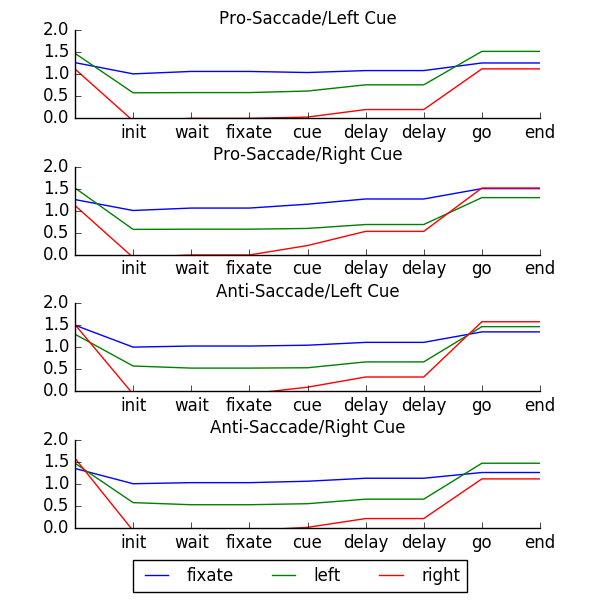
\includegraphics{figure_saccade.png}
\caption{Q-value units' Activity for the Saccade/Anti-saccade Task
(reproduction of figure 2D). The ``Fixate'' action dominates until the
``Go'' phase where the model correctly chooses the direction to look at.
As in the reference article, there is a noticeable reaction after the
``Cue'' phase.}\label{fig:saccade}
\end{figure}

\begin{figure}
\centering
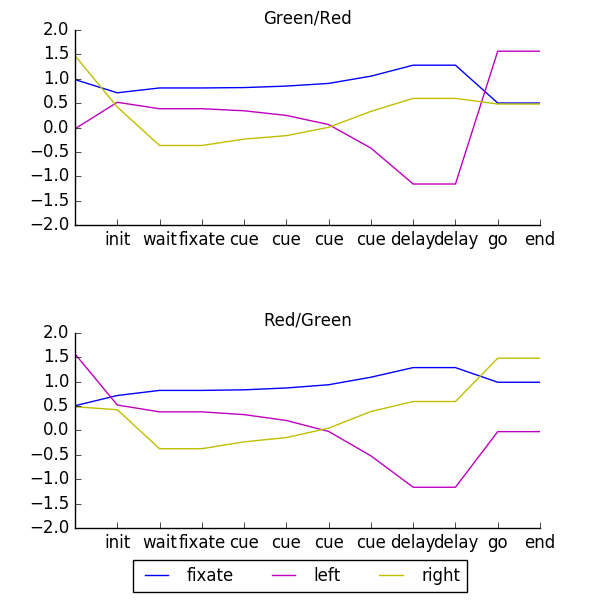
\includegraphics{figure_probabilistic.png}
\caption{Q-value units' Activity for the Probabilistic Decision Making
Task (reproduction of figure 4C). For both trials, the green target in
the best choice. Once again, the model maintains fixation until the
``Go'' phase where it makes the correct
decision.}\label{fig:probabilistic}
\end{figure}

\section{Conclusion}\label{conclusion}

The results obtained are comparable to those announced in the article.
Ambiguities in the experiments' descriptions could be the cause for
worse performances, but do not contradict the article's overall
conclusion.\\

{\sffamily \small
  \printbibliography[title=References]
}
\end{document}
